\section{Background}
\label{sec:background}
This section presents a brief history of traffic routing problem and the selfish routing model, defining the terminology and context in which 
we describe later results.

\subsection{The Traffic Routing Problem}
Traffic routing problems naturally arise in communication or transportation networks, where users are trying to minimize the latency that they or their data experiences. Users make these decisions only with their own traffic in mind.
However, links in the network often become \emph{congested} if too many users decide to route their data 
or cars through that link. Consequently, in these networks, the path each user chooses can affect the travel times of other
users. Here, we describe Roughgarden and Tardos' formalization of the problem of minimizing latency in terms of multicommodity flow networks~\cite{tardos,roughgarden}, and use Pigou's example network in Figure~\ref{fig:Pigou} as a running example. In this graph, one path has a constant latency while the other path's latency increases with the number of users using it. We will later use this to reason about how much latency increases from optimum when users make selfish routing decisions. We will also briefly reference Braess's graph (Figure~\ref{fig:braess}) in which the outer edges have similar latency functions to the Pigou network while the middle edge has a latency of $0$.

%These are used even by selfish users as long as the middle edge isn't introduced, but once the middle edge is introduced, everyone uses it increasing the overall latency as well as per-user latency.

\begin{figure}[ht!]
    \centering
\begin{minipage}{0.45\textwidth}
    \centering
    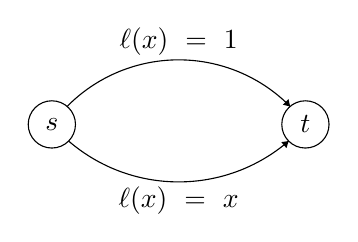
\begin{tikzpicture}[scale=0.1]
    \tikzstyle{every node}+=[inner sep=0pt]
    \draw [black] (18,-17.9) circle (3);
    \draw (18,-17.9) node {$s$};
    \draw [black] (50.2,-17.9) circle (3);
    \draw (50.2,-17.9) node {$t$};
    \draw [black] (19.94,-15.615) arc (135.3471:44.6529:19.905);
    \fill [black] (48.26,-15.62) -- (48.05,-14.69) -- (47.34,-15.4);
    \draw (34.1,-9.2) node [above] {$\ell(x)\mbox{ }=\mbox{ }1$};
    \draw [black] (48.072,-20.011) arc (-49.23907:-130.76093:21.4);
    \fill [black] (48.07,-20.01) -- (47.14,-20.15) -- (47.79,-20.91);
    \draw (34.1,-25.7) node [below] {$\ell(x)\mbox{ }=\mbox{ }x$};
    \end{tikzpicture}
    \caption{Pigou's example traffic routing problem, with a demand of $r_{(s,t)} = 1$}
    \label{fig:Pigou}
\end{minipage}
\hspace{1cm}
\begin{minipage}{0.45\textwidth}
    \centering
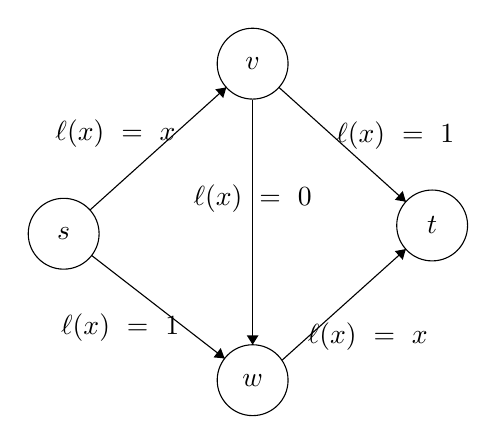
\begin{tikzpicture}[scale=0.15]
\tikzstyle{every node}+=[inner sep=0pt]
\draw [black] (26.7,-28.8) circle (3);
\draw (26.7,-28.8) node {$s$};
\draw [black] (57.9,-28.1) circle (3);
\draw (57.9,-28.1) node {$t$};
\draw [black] (42.7,-14.4) circle (3);
\draw (42.7,-14.4) node {$v$};
\draw [black] (42.7,-41.2) circle (3);
\draw (42.7,-41.2) node {$w$};
\draw [black] (29.07,-30.64) -- (40.33,-39.36);
\fill [black] (40.33,-39.36) -- (40,-38.48) -- (39.39,-39.27);
\draw (31.49,-35.5) node [below] {$\ell(x)\mbox{ }=\mbox{ }1$};
\draw [black] (28.93,-26.79) -- (40.47,-16.41);
\fill [black] (40.47,-16.41) -- (39.54,-16.57) -- (40.21,-17.31);
\draw (31.09,-19.09) node [below] {$\ell(x)\mbox{ }=\mbox{ }x$};
\draw [black] (42.7,-17.5) -- (42.7,-38.2);
\draw (42.7,-27) node [above] {$\ell(x)\mbox{ }=\mbox{ }0$};
\fill [black] (42.7,-38.2) -- (43.2,-37.4) -- (42.2,-37.4);
\draw [black] (45.2,-39.5) -- (55.67,-30.1);
\draw (57.58,-37.5) node [left] {$\ell(x)\mbox{ }=\mbox{ }x$};
\fill [black] (55.67,-30.1) -- (54.74,-30.27) -- (55.41,-31.01);
\draw [black] (44.93,-16.41) -- (55.67,-26.09);
\fill [black] (55.67,-26.09) -- (55.41,-25.18) -- (54.74,-25.93);
\draw (54.78,-21.74) node [above] {$\ell(x)\mbox{ }=\mbox{ }1$};
\end{tikzpicture}
\caption{Braess's graph for the traffic routing problem where the addition of the center edge inadvertently increases the overall latency.}
\label{fig:braess}
\end{minipage}
\end{figure}



\medskip\noindent
\textbf{The input} $(G,r,\ell)$ to a traffic routing problem consists of:
\begin{itemize}
    \item A network $G = (V, E)$ of $|V|$ destinations (e.g., locations or servers) and $|E|$ links 
     \item A set of $k$ source-destination pairs $S=\{(s_1,t_1), \cdots (s_k,t_k)\}$ representing traffic demands
    \item A {rate} $r_i$ of traffic for each $(s_i,t_i)\in S$ representing the traffic demand from $s_i$ to $t_i$
    \item A {latency} function $\ell$ that assigns a per-edge function $\ell_e$ to each edge $e$ describing how adding traffic (i.e., congestion) to $e$ affects the time taken to travel across $e$. We can also think of $\ell$ as assigning per-path latencies: for any path $p$ in the graph that carries flow $f$,
        $\ell_p(f) = \sum_{e\in P}\ell_e(f_e)$.
        We assume that $\ell$ is continuous, nonnegative, and nondecreasing.
\end{itemize}
In Figure~\ref{fig:Pigou}, we see a single source-destination input network with an example (linear) cost function with $r_{(s,t)} = 1$.

\medskip\noindent
\textbf{Solutions} correspond to flow assignments to the set of simple paths $P_i$ between $s_i$ and $t_i$ for all $i$. Note that our solutions assume \emph{nonatomic} entities: the flows we find may not be integral.
Intuitively, this means that the demand from one $s_i$ to $t_i$ is generated by an infinite number
of entities in the network, which allows us to reason about continuous, rather than discrete, functions.
%
We can describe a flow assignment $f$ via use its path decomposition ($f$ is made up of flows $f_p$, the flow on a single path $p \in P_i$, where $f_p$ flow is added to all edges in $p$); alternatively, we can describe the flow on each edge $f_e = \sum_p \sum_{e\in p} f_p$, (equal to the sum of flow on all paths that use $e$).

A \emph{feasible} solution given such an input is an assignment of path flows such that the demand from $s_i$ to $t_i$ is met:
$$\forall 1 \le i \le k,~\sum_{p\in P_i} f_p = r_i$$
%
An \emph{optimal} (feasible) solution given such an input is the feasible flow assignment $f$ that minimizes the \textbf{social welfare latency cost} $C(f)$, where
$$C(f) = \sum_i\sum_{p\in P_i}\ell_p(f)f_p = \sum_{e\in E} f_e\ell_e(f_e)$$

Intuitively, we are calculating the latency of each path of a given flow assignment, weighing 
each path's latency proportional to the amount of flow through that path. More concretely,
if we were to let flow represent the routes chosen by (infinitely many) users, $C(f)$ calculates the average latency over all users. Thus, when minimizing $C(f)$, some users may incur 
more latency so that other users can go faster: the optimal flow is the \emph{socially optimal} solution.
Note that there exists an optimal flow $f^*$ minimizing $C(f)$ because we assume $\ell$ is continuous and the set of feasible flows is compact.

In our running example (Figure~\ref{fig:Pigou}), a feasible flow is any flow that sends one unit from $s$ to $t$ (divided in any fashion between the top and bottom edges).
The optimal flow is the flow that sends half the traffic through the lower edge and half through the upper edge: the users on the lower edge only experience a latency of $1/2$, while the users on the upper edge experience a latency of $1$, making the social welfare cost cost $3/4$.

\subsection{Coordination Models and the Price of Anarchy}
Before we can create algorithms to solve the traffic routing problem, we must first assume a \emph{coordination model} for our traffic network.
There are two clear extremes: (1) centralized control, in which some entity (e.g., an air traffic controller) knows all traffic demands and latencies and routes accordingly, and
(2) decentralization, i.e., a complete \emph{lack} of coordination between
entities in the network.
In a centralized setting, there is a clear optimal solution, as shown in the previous section.
However, in a decentralized and uncoordinated model, the lack of coordination and the exercise of free will in accordance to individual motives can result in
inefficiencies. 

\medskip
\textbf{The Price of Anarchy} (PoA) allows us to measure the inefficiencies of a decentralized model, and was first introduced by Koutsoupias and Papadimitriou in 1999~\cite{poa}. 
We treat the decentralized model as a game in which each individual optimizes for her own \textbf{individual cost function $c$}, allowing us to compute the achieved flow at the resulting Nash equilibrium (proven to exist if the cost functions are continuous)~\cite{wardrop,haurie,beckmann1956studies}.
The price of anarchy $\rho(G,r,\ell)$ is defined as the ratio between the social welfare latency cost at the flow $f$ achieved at Nash equilibrium, and the optimally minimal social welfare latency cost $C(f^*)$, $\rho(G,r,\ell) =\frac{C(f)}{C(f^*)}$.
(This is similar to how we measured the distance from optimal of an approximation algorithm in a limited computational power model, and of online algorithms in an incomplete information model.)

The set of flows at Nash equilibrium are defined such that for all $i$ source-destination pairs, all the paths from $s_i \to t_i$ have the minimum-possible cost with respect to an individual's cost function $c$. In other words, the (nonzero) flow paths at Nash equilibrium have equal path costs, and no user could decrease her cost by choosing a different path:
$$\forall 0\le i \le k,~\forall p_1, p_2\in P_i~s.t.~f_{p_1} > 0~\text{and} f_{p_2} > 0,~ c_{p_1}(f) = c_{p_2}(f)$$
Note that this corresponds exactly to the solutions to the following (convex) program solvable in polynomial time:
$$NE = \min_f\Big(\sum_e \int_0^{f_e} c_e(t)dt\Big) \text{ subject to feasibility constraints}$$
whereas the flow optimizing the social welfare latency cost corresponds exactly to the (polynomial-time) solutions to the following (convex) program: 
$$SW = \min_f\Big(\sum_e f_e\ell_e(f_e)\Big) \text{ subject to feasibility constraints}$$

\subsection{The Selfish Routing Model}
One example of an uncoordinated model is the \emph{selfish routing} model, in which all entities in the network are selfish and choose a route minimizing their individual latency without caring (or knowing) about the effects on other users~\cite{tardos}.
The selfish routing model corresponds to flows at a Nash equilibrium where each user optimizes her individual cost function
$c^s(f) = \ell(f)$.
Thus, the program optimized at Nash equilibruim is
$$NE = \min_f\Big(\sum_e \int_0^{f_e} \ell_e(t)dt\Big) \text{ subject to feasibility constraints}$$

If we revisit our running example in Figure~\ref{fig:Pigou}, we note that the flow at Nash equilibrium corresponds to a flow that sends the entire unit of traffic through the bottom edge (the 0 flow through the top path has latency 1, and the unit flow through the bottom path will have latency 1).
Intuitively, each user routing from $s$ to $t$ will selfishly choose to take the bottom route because she will reason that the bottom route can have latency no worse than the top route. However, when all the users apply this same strategy, the bottom route becomes more congested and leads to a total average latency $C(f) = 1$.
Thus, in Figure~\ref{fig:Pigou}, the price of anarchy $\rho$ is $\frac{1}{3/4} = \frac{4}{3}$. A similar problem plagues Figure~\ref{fig:braess} too in that the outer paths are optimal and used by selfish users too as long as the 
middle low latency edge isn't introduced. However, once it is reduced, all users believe they can reduce their latency by using that edge and in essence, everyone's latency increases because they all use a single path through that
edge.

We next describe and present the main results regarding the price of anarchy in this (decentralized) selfish routing model, which will act as a basis to which we will compare traffic routing results in more recently formulated models.

\subsection{Main Results}
\begin{theorem}
    If $f$ is a flow at Nash equilibrium for a given input $(G, r, \ell)$ and $f^*$ is a feasible flow for $(G, 2r, \ell)$, then $C(f) \leq C(f^*)$
\end{theorem}

\begin{proof-sketch}
    This result demonstrates that the latency incurred when users selfishly route $r$ units of flow is at most the optimal (minimum) latency when routing twice as much demand ($2r$).

\begin{figure}[t!]
    \centering
    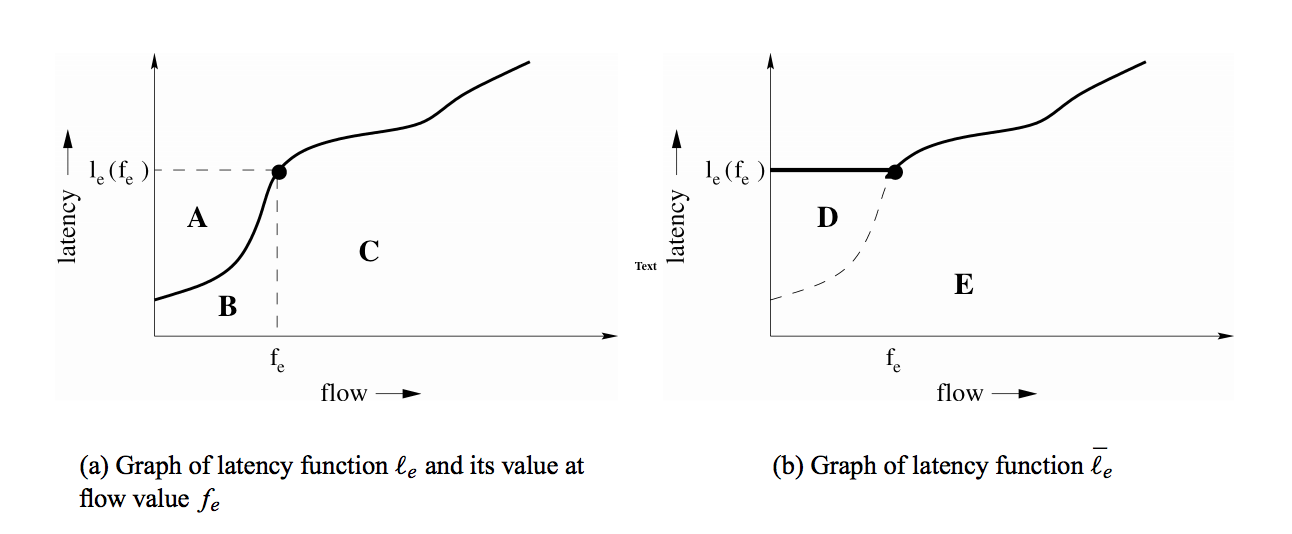
\includegraphics[width=.7\textwidth]{graph}
    \caption{Visualizing latency costs of individual edges}
    \label{fig:thm1}
\end{figure}

    For any Nash equilibrium solution $f$ for $(G, r, \ell)$ and any feasible solution $f^*$, we can draw a figure like Figure~\ref{fig:thm1} for each edge $e$ in $G$, where $A,~B,~C,~D,\text{ and } E$ represent the magnitude of the areas of the indicated portions of the graph.
    $A+B$ represents the latency cost $C(f)$ of the Nash equilibrium solution $f$ for $(G, r, \ell)$, and $B+C$ represents the cost $C(f^*)$ of the feasible solution $f^*$ for $(G, 2r, \ell)$. $D$ and $E$ together represent the
    cost of a flow $f^*$ under a modified latency function $\bar{l_e}$ as depicted.
    
    Since $D+E \le D+B+C$, and $D < A+B$, we know that $D+E-(B+C)\le D \le A+B $. This means that $B+C\ge D+E -(A+B)$. On the other hand $D+E\ge 2(A+B)$ (reason below). Therefore, we have that $C(f^*)=(B+C)\ge 2(A+B)-(A+B)= A+B= C(f)$. 
    This indicates that the latency of any Nash equilibrium flow for $(G, r, \ell)$ is no bigger than represents the latency of any feasible solution for $(G, 2r, \ell)$.
    
    The main idea of the proof for this theorem lies in that the subset if the area $C$ is at least as big as the area $A+B$. This is always true because the latency $\bar{\ell}_e$ is a nondecreasing function and thus the graph of latency function gives a shape that looks like a generalized trapezoid (in particular, a right generalized trapezoid lying on the horizontal axis). 
    %Then we can obtain the result based on the property of a trapezoid shape. Therefore, the cost of any feasible solution for $(G, 2r, \ell)$ is at least twice the cost $C(f)$ of any Nash equilibrium solution for $(G, r, \ell)$. Then the area under the black line from $0$ to $2f_e$ in subgraph (a) is at least $2C(f)-C(f)$ and thus larger than $C(f)$. 
   %The cost of any feasible solution for $(G, 2r, \ell)$, and the area under the black line from $0$ to $2f_e$ in subgraph (b) is at most $C(f)$ more than the cost of any feasible solution for $(G, 2r, \ell)$, and the area under the black line from $0$ to $2f_e$ in subgraph (a). So the area of the generalized trapezoid under the black line from $0$ to $2f_e$ is more than two times the area under the black line on the left side of $f_e$ in subgraph (b). 
    %$+E$ under the black line from $0$ to $2f_e$ in subgraph (b) represents the cost of any feasible solution for $(G, 2r, \ell)$. The area under the black line on the left side of $f_e$ in subgraph (a) represents the cost $C(f)$ of any Nash equilibrium solution for $(G, r, \ell)$. Note that since the area of t he area under the black line on the left side of $f_e$ in subgraph (a) is at least half of the dashed line, we know that the cost of any feasible solution for $(G, 2r, \ell)$, and the area under the black line from $0$ to $2f_e$ in subgraph (b) is at most $C(f)$ more than the cost of any feasible solution for $(G, 2r, \ell)$, and the area under the black line from $0$ to $2f_e$ in subgraph (a). So the area of the generalized trapezoid under the black line from $0$ to $2f_e$ is more than two times the area under the black line on the left side of $f_e$ in subgraph (b).
    % Vibhaa: might be helpful to add line segments/naming to the figure - also not sure if the black line on left side needs to be half of dashed line. Check 
    %also check notation
\end{proof-sketch}

\begin{theorem}
    If the edge latency functions are linear, i.e., $\ell_e = a_ef_e + b_e$ for every edge $e \in E$, then $\rho(G, r,\ell) \leq 4/3$.
    \label{thm:linear}
\end{theorem}

\begin{proof-sketch}
    The latency of any flow $x$ under these edge latency functions is $C(x) = \displaystyle \sum_e a_ex^2_e + b_ex_e$.

    Let's consider two flows $f$ and $f^*$ such that $f$ is at Nash equilibrium in $(G, r, \ell)$ and $f^*$ is the flow optimizing the social welfare cost of $G,r,\ell)$. We first consider optimally routing the first $r/2$ demand 
    across all source-destination pairs. It turns out that $f/2$ is optimal for $(G, r/2,\ell)$ when the edge latency functions are linear. This can be derived from the fact that paths with
    non-zero flow at a Nash equilibrium have the same path latency while paths with non-zero flows at the global optimum have the same marginal cost of increasing the flow. Now, if we look at the cost
    $C(f/2)$ of routing this in terms of the latency of routing the flow $f$ at Nash equilibrium, we notice that $C(f/2) = \displaystyle \sum_e \frac{1}{4}a_ef^2_e + \frac{1}{2}b_ef_e \geq \frac{1}{4}C(f)$
    from the above cost expression. Thus, in other words, routing the first $r/2$ optimally has a latency that is at least one-fourth of the latency of the Nash equilibrium flow.
    %% Do we need the actual proof of the fact that $f/2$ is optimal for the half rate case - we could also just reference Lemmas 4.1 and 4.3?

    This leaves the remaining $r/2$ that needs to be routed optimally to route $f^*$ fully. To reason about this, let's look at a small $\delta r_i$ increase in flow from $s_i$ to $t_i$ that already carries $x$ units 
    of flow. For a convex latency function, we expect the increase in latency to be at least $\delta r_i\ell'(x)$ where $\ell'$ if the minimum marginal increase in $C$. If we consider starting at the 
    optimal flow $f/2$ for the $r/2$ demand and increasing the flow on each path by a small $\delta r_i$, the subsequent increase in 
    latency across be all paths can be summed as  $\displaystyle \sum_{i = 1}^k\ell'(f/2)\delta r_i$. In particular, for linear edge latency functions, the marginal increase in latency on every edge at $f/2$ is exactly
    the latency of that edge at $f$. Thus, $\ell_e'(f/2) = \ell_e(f)$. We now know that when we set $\delta = 1$ and increase the rate by $r_i/2$ on every $s_i$, the overall increase in latency is at least $\displaystyle \frac{1}{2}\sum_{i= 1}^k\ell(f)r_i = \frac{1}{2}C(f)$. The last part is by definition of $C(f)$. 
    
    We have shown that routing the first $r/2$ demand optimally costs at least $C(f)/4$ and the next $r/2$ when augmented, costs at least another $C(f)/2$. In total, the cost $C(f^*)$ associated with the optimal is at least $\frac{3}{4}C(f)$. In other words,
    the flow at Nash equilibrium has cost utmost $\frac{4}{3}C(f^*)$ where $f^*$ is the flow achieving optimal latency.
\end{proof-sketch}
